\chapter{Modelo proposto}\label{cap:proposta}
Este capítulo abordará o sistema de treinamento proposto, será exposto como funciona todo o ambiente simulado. Dentre os módulos que compõe um veículo autônomo o foco deste projeto será em desenvolver o componente de controle de deslocamento que é responsável por fazer carro percorrer um trajeto. No mundo real as rotas seriam geradas por outro componente, porém isto está além do escopo deste projeto, portanto elas serão definidas pelo autor. Importante ressaltar que o conjunto de rotas deve ser composto por uma variedade de trajetos que exijam uma diversidade de manobras a serem aprendidas pelo agente.

% Esta seção está sujeita a mudanças feitas no ambiente durante o PGCIII. 
\section{Modelo}\label{modelo}
Aqui é descrito sobre o modelo do projeto. Por "modelo" entende-se o conjunto ambiente-agente-recompensas. Cada um deles é detalhado nas subseções abaixo.

\subsection{O ambiente}
A simulação envolve em treinar o veículo para percorrer trajetos em ambiente urbano, a princípio, por uma questão de simplicidade o agente não terá de lidar com declives ou aclives, semáforos, outros veículos ou pedestres. Porém outros elementos estáticos comuns de uma cidade como calçadas, postes, árvores, prédios, etc. Portanto, o foco poderá se manter no estudo de fazer um agente percorrer as rotas. Às bordas do cenário há muros que limitam o alcance do veículo, foi concluído pelo autor que o tamanho atual é suficiente para os treinos iniciais, em estudos futuros pode ser considerado a expansão do cenário. O agente recebe uma punição ao se chocar com a calçada ou com os muros da borda da cidade.

\begin{figure}[h]
   \centering
   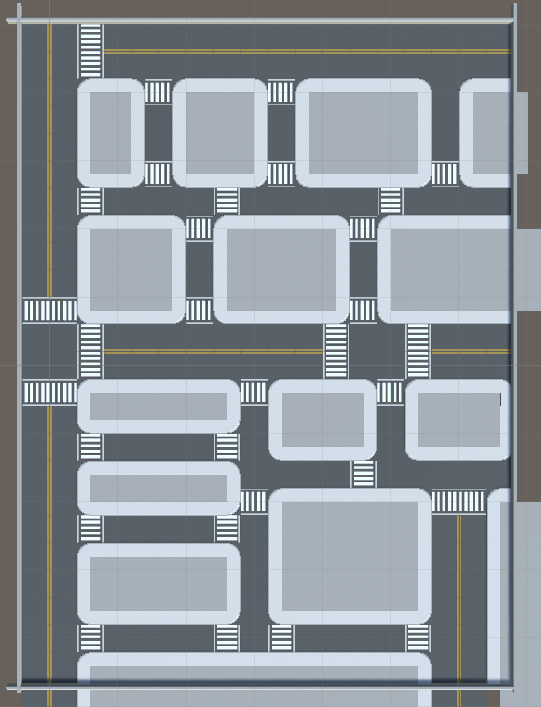
\includegraphics[scale=0.45, angle=90]{figs/Mapa-simulador-visao-superior.png}
    \caption{Visão superior o cenário urbano criado para o treinamento do veículo}
    \label{fig:map-view}
 \end{figure}

As rotas são compostas por: origem, \textit{checkpoints} e destino. O primeiro indica o local de partida do veículo, o último é o objetivo final do agente naquele episódio. Os \textit{checkpoints} são barreiras que indicam o caminho que deve ser percorrido, cada vez que o veículo atravessa uma delas ele ganha uma recompensa, isto é uma forma de indicar a ele que está fazendo o correto. Há 17 percursos predefinidos, cada uma delas possuem características distintas como distância origem-destino, quais e quantas conversões a serem feitas, isto foi moldado visando trazer uma diversidade maior de desafios a serem superados pelo agente. Assim como o tamanho do cenário, novos trajetos podem ser considerados em estudos futuros.

\begin{figure}[h]
   \centering
   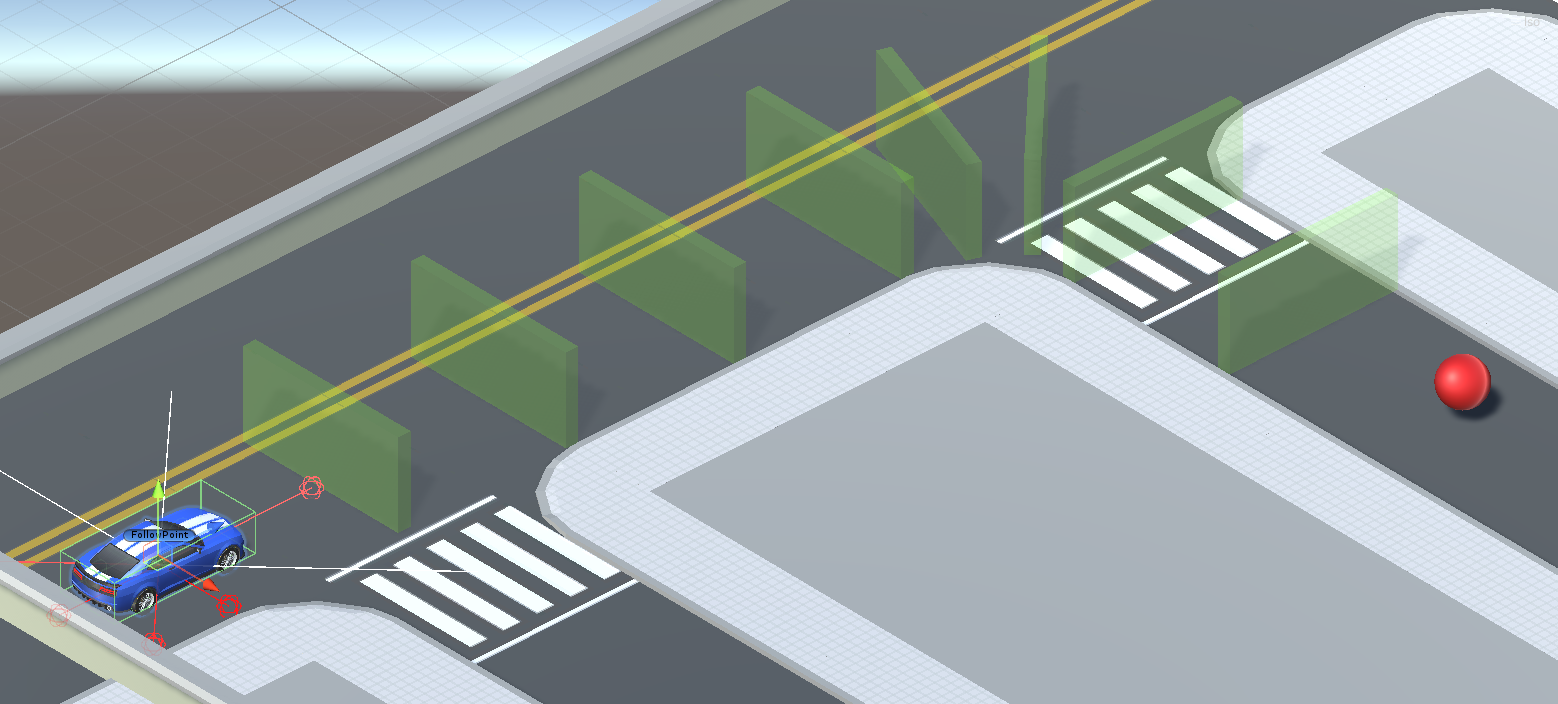
\includegraphics[scale=0.35]{figs/detalhe-rota.png}
    \caption{Rota vista de perspectiva isométrica, o agente posicionado a origem ao canto esquerdo, com os \textit{checkpoints} ao longo do percurso até o destino no canto direito.}
    \label{fig:route-view}
 \end{figure}

 \subsection{O agente}
 Para o aprendizado o veículo possui 8 sensores apontando para todas as direções uniformemente espaçadas, estes sensores são um \textit{component} do pacote \textbf{ML-agents} da Unity3D, são capazes de medir a distância dos objetos próximos ao veículo e também são capazes de distinguir quais são estes objetos. Estes sensores dentro do editor são representados por feixes que partem do centro do veículo, é possível configurar diversos atributos deles como a quantidade, o ângulo máximo de distância do primeiro ao último, o ângulo vertical (que indica se eles apontam para cima ou para baixo) e o tamanho da esfera, que nada mais é que a tolerância de colisão do sensor.

 \begin{figure}[h]
   \centering
   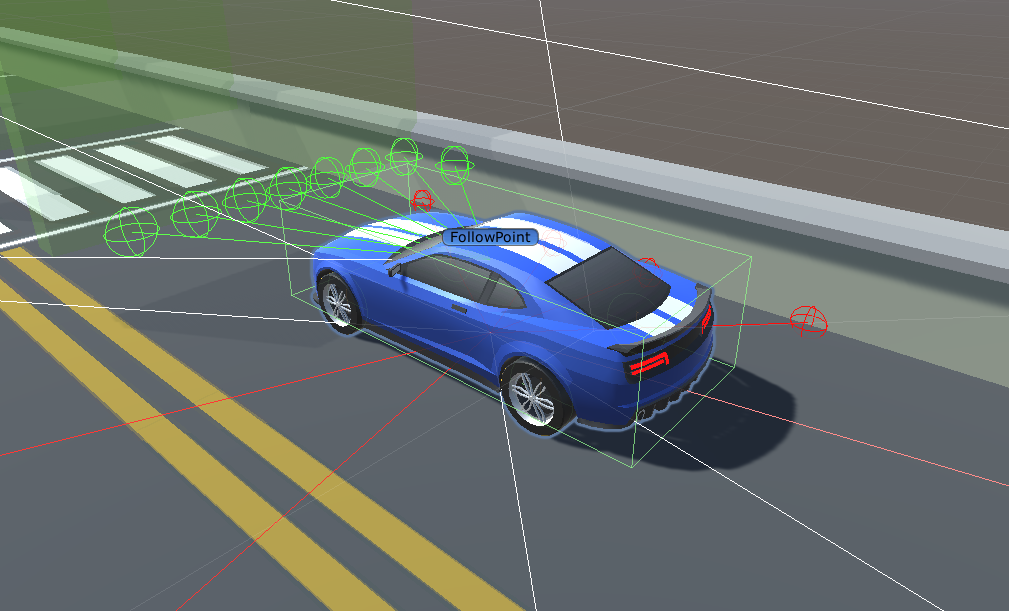
\includegraphics[scale=0.35]{figs/agente-raios-checkpoint.png}
    \caption{Exemplo do agente e seus raios perceptores, é possível ver 6 raios laterais se chocando com as calçadas ao lado, o raio frontal se chocando com o \textit{checkpoint}.}
    \label{fig:casting-rays}
 \end{figure}

 Além dos sensores, foi adicionado a velocidade do veículo a lista de observações do agente. Vale lembrar que o não foi implementado um recurso de imagem em um primeiro momento, ou seja, o veículo só enxerga através dos sensores e tem ciência de sua própria velocidade, ele é "cego" a qualquer outro elemento do ambiente que não esteja se choccando com o sensor.

 Quanto as ações que o agente pode fazer são apenas 3: acelerar, frear e direcionar as rodas a direita e a esquerda. A primeira e a última ação são chamadas ações contínuas, sendo assim um número que indica o nível de aceleração que o carro irá produzir, e no caso da direção da roda o quão direciona elas estão a esquerda ou direita. O ato de frear por outro lado é uma grandeza discreta, o veículo está ou não está freando.

\subsection{As recompensas}
Dado os sensores do agente e o ambiente montado podemos definir as recompensas/punições das seguintes ocorrências: chegar ao destino ($R_d = 1$, sempre), atingir um \textit{checkpoint} ($R_c$), colidir com a/subir na calçada ($P_c$), colidir com a parede($P_p$), não chegar no destino a tempo($P_t$). Além disso temos os seguintes cenários possíveis: o agente chega ao destino, o agente não chegar a tempo, o agente tombar o veículo. As recompensas estão no intervalo $[-1,1]$ e serão aplicadas da seguinte forma em cada cenário:

\begin{itemize}
   \item Chega ao destino: $R_T = R_d - P_c - P_p$
   \item Não chega a tempo: $R_T = R_c - P_c - P_p$
   \item Tomba o carro: $R_T = -1$
\end{itemize}

\section{Os algoritmos e hiper-parâmetros}\label{algoritmos}
Para executar o treino é necessário especificar para o \textbf{ml-agents} o algoritmo e suas configurações, para isso existe um arquivo \textbf{.yaml} que é responsável por isso. Abaixo, um exemplo seguido da explicação de cada parâmetro:

\begin{lstlisting}
behaviors:
   MoveToTarget:
      trainer_type: ppo
      max_steps: 9600000
      time_horizon: 64
      summary_freq: 60000
      keep_checkpoints: 16     
      checkpoint_interval: 600000
      hyperparameters:
         learning_rate: 1.0e-5
         batch_size: 1024
         buffer_size: 10240
         beta: 5.0e-2
         epsilon: 0.1
         lambd: 0.99
         num_epoch: 8
         learning_rate_schedule: linear
         beta_schedule: linear
         epsilon_schedule: linear
      network_settings:
         normalize: false
         hidden_units: 64
         num_layers: 2
      reward_signals:
         extrinsic:
            gamma: 0.99
            strength: 1.0
\end{lstlisting}

O arquivo começa com o \textbf{behaviors} que é uma lista de configurações dos comportamentos do agente, neste projeto haverá apenas um que é chamado \textbf{MoveToTarget}. Abaixo segue uma lista dos hiper-parâmetros mais relevantes, o texto aqui é em grande parte traduzido da documentação oficial do \textbf{ml-agents} (\citeonline{juliani2020}) com algumas remoções de informações não relevantes pra este projeto e com alguns adendos do autor caso necessário.

\begin{description}
   \item [trainer\_type:] O algoritmo que será usado, neste projeto serão PPO ou SAC
   \item [max\_steps:] O número máximo de passos(observações coletadas e ações tomadas pelo agente) tomados  no ambiente. No simulador a tarefa sempre será episódica, o tamanho do episódio pode variar nos ajustes, mas cada um possui em torno de 1200 \textit{steps}.
   \item [time\_horizon:] O número de \textit{steps} anteriores a ser coletado por agente para adicionar ao \textit{buffer} de experiência. Quando este limite é alcançado antes do fim de um episódio, um valor estimado é usado para prever a expectativa geral de recompensa a partir do estado atual do agente. Por isso, esse parâmetro varia entre menos enviesado mas com alta variância estimada (longo prazo) e mais enviesado mas com estimativa de menor variância (curto prazo). Em casos onde há frequente sinais de recompensas ou em episódios muito longos, um número menor pode ser mais ideal.
   \item [hyperparameters->learning\_rate:] Taxa inicial do salto a cada atualização do gradiente descendente. Este número geralmente deve diminuir com se o treino está instável e a recompensa com aumenta consistentemente.
   \item [hyperparameters->batch\_size:] O número de experiências coletadas para cada atualização do gradiente descendente. Em caso de usar ações contínuas ele deve estar na casa do milhares, caso contrário na casa das dezenas deve bastar.
   \item [hyperparameters->batch\_size:] Número de experiências a ser coletada antes de atualizar o modelo da política. Tipicamente, um buffer size maior corresponde a um treino mais estável. No caso do SAC este número deve ser milhares de vezes maior que um episódio típico, pois o algoritmo deve aprender de experiências velhas quanto mais novas.
   \item [hyperparameters->beta:] (somente PPO) força da regularização da entropia, que faz com que a política seja "mais aleatória". Isto garente que o agente explore apropriadamente o espaço da ação durante o treino. Aumenta-lo faz com que o agente tome mais ações aleatória. Isto deve ser ajustado de modo que o a entropia (medido pelo tensorboard) lentamente decresça conforme aumenta a recompensa. Se a entropia cair muito rápido aumente o \textbf{beta}, caso demore demais diminua-o.
   \item [hyperparameters->epsilon:] (somente PPO) Influencia no quão rapidamente a política pode evoluir durante o treino. Corresponde ao limite da divergência entre as velhas e novas políticas durante a atualização do gradiente descendente. Um valor menor leva a atualizações mais estáveis, mas deixa o processo de aprendizagem mais lento.
   \item [hyperparameters->lambd:] (somente PPO) parâmetro de regularização (lambda) usado quando calculado o estimador de valor generalizado (GAE (\citeonline{1506.02438})). Isto pode ser entendido em o quanto o agente depende no seu atual valor estimado quando atualizando o valor estimado. Valores baixos corresponde a apoiar-se mais no valor atual (alto viés/\textit{bias}) e valores elevados corresponde a confiar mais nas recompensas recebidas pelo ambiente (que pode causar alta variância). (geralmente varia de 0,9 a 0,99)
   \item [hyperparameters->num\_epoch:] (somente PPO) O número de passagens a fazer pelo buffer\_size quando otimizando gradiente descendente. Este deve crescer semelhante ao batch\_size. Diminui-lo tende a ter atualizações mais estáveis, aumentá-lo tem-se um treino mais lento. (geralmente varia entre 3 a 10)
   \item [hyperparameters->learning\_rate\_schedule:] Determina se o valor do learning\_rate muda durante o treino, os valores podem ser \textit{linear} ou \textit{constant}. Sendo o primeiro ele irá decair linearmente até zero quanto executar o \textit{max\_steps}. O segundo mantém o valor constante. É recomendado adotar \textit{linear} para PPO e o outro quando usar SAC.
   \item [hyperparameters->beta\_schedule:] (somente PPO) Similarmente ao acima mas para o \textbf{beta}. 
   \item [hyperparameters->epsilon\_schedule:] (somente PPO) Similarmente ao acima mas para o \textbf{epsilon}. 
   \item [hyperparameters->buffer\_init\_steps:] (somente SAC) Número de experiências a coletar no buffer antes de atualizar o modelo da política. Inicialmente o buffer é preenchido com ações aleatórias,o que é muito útil para exploração. Este número deve ser na casa de dezenas de vezes maior que um típico episódio.
   \item [hyperparameters->init\_entcoef:] (somente SAC) Corresponde a entropia inicial definida no começo do treino e é o quanto o agente deve explorar inicialmente. No SAC, o agente é incentivado a tomar decisões aleatorias a fim de explorar melhor o ambiente. O coeficiente de entropia é ajustado automaticamente para um valor alvo predefinido então o \textit{init\_entcoef} é apenas o valor inicial. Quanto maior o valor maior a exploração inicial. Para ações contínuas o típico valor está no invervalo 0,5-1,0, discreto em 0,05-0,5.
   \item [network\_settings->hidden\_units:] O número de nós em cada camada intermediária da rede neural totalmente conectada (valores típicos giram em torno de 32 a 512).
   \item [network\_settings->num\_layers:] O número de camadas intermediárias na rede neural (tipicamente tem valor de 1 a 3).
   \item [network\_settings->normalize:] Se normalização deve ser aplicada no vetor de observação. Esta normalização pode melhorar o treino em caso de tarefas que lidam com controles contínuos complexos, mas pode atrapalhar caso contrário.
\end{description}

\section{Metodologia}
A tarefa a ser resolvida pelo agente é episódica, onde em cada episódio ele terá que chegar ao destino seguindo o trajeto definido pelos checkpoints. O episódio só acaba se ele atingir o destino ou se tombar o veículo. Durante o treino o agente receberá um trajeto aleatório em cada episódio e durante o teste o agente terá que percorrer três vezes todos trajetos na ordem de cada um deles no projeto da Unity. No final terá o desempenho dele no teste será medido tanto quantitativamente quanto dissertativamente. Quantitativamente pois será mostrado o desempenho em cada rota, quantidade (de 0 a 3) de que conseguiu chegar ao destino em cada um deles e quantas colisões foram registradas no total. Dissertativamente será a análise textual com opnião do autor sobre a condução do veículo e focará em observar características mais subjetivas (por exemplo se o agente conduz o carro com muitas revoluções ou se acelera e freia muito bruscamente, entre outras). 

Como foi dito na seção \nameref{sec:objetivos}, o propósito deste projeto é estudar a criação e desenvolvimento de um ambiente simulado para o treino de veículo autônomos, logo o mesmo está sujeito a mudanças e melhorias para tornar a simulação o mais próximo da realidade possível. O versionamento do modelo será definido aqui, suas mudanças mais relevantes serão detalhadas e justificadas, mudanças estas que incluem alterações de recompensas, observações do agente, hiper-parâmetros dos algoritmos PPO e SAC. Vale ressaltar que as mudanças seguem na ordem da maior pra menor: alteração do agente ou ambiente, reorganização das recompensas, ajustes nos hiper-parâmetros. Não são todos os ajustes que serão expostos aqui, especialmente ao dos hiper-parâmetros, se um alteração não levar a um resultado diferente antes de outro reajuste então pode ser considerado insignificante.

\subsection{Treinamento e teste}
Tendo o \nameref{modelo} e \nameref{algoritmos} detalhados acima é preciso explicar o treinamento e teste. O treinamento é executado via linha de comando, é necessário ativar o ambiente Python, gerar um executável do simulador pelo editor da unity e ter um arquivo de configuração do algoritmo. Tendo estes três itens é possível executar o comando do ml-agents e por o agente em treino. Após o treino finalizar é gerado um arquivo \textbf{.onnx} que é política final do agente, a rede neural com os coeficientes gerados pelo algoritmo após o treino, o seu "cérebro". Finalmente podemos por o agente em teste, de volta ao editor da Unity3D, basta carregar o cérebro no agente e executar o teste, o veículo agora se mexe sozinho sem input do usuário, e o mesmo deve estar agindo de acordo com os resultados do treino, seja ele um sucesso ou não.

Nos testes o agente deverá percorrer os mesmos trajetos, agora eles não serão aleatórios, ele percorrerá cada um três vezes. Como na lista de observações não inclui qualquer informação sobre qual trajeto ele está percorrendo no momento, o autor não viu necessidade de separar trajetos de treino e de teste, embora essa possibilidade posta em estudos futuros.

\subsubsection*{Estatísticas de treino}
Quando o treino é finalizado é armazenado diversas estatísticas que são exibidas pelo \textbf{tensorboard}. Nelas é possível ter uma visualização do desempenho do agente durante o treino e sua curva de aprendizado. As que serão analisadas e discutidas na próxima parte estão descritas na lista abaixo. Assimi como a listagem dos hiper-parâmetros essas definições são traduções diretas da documentação do ML-agents (\citeonline{juliani2020}).

\begin{description}
   \item [Cumulative Reward:] A mediana da recompensa acumulada no episódio do agente. Deve aumentar ao longo de um treino bem sucedido (Esta estatística possui dois gráficos, um de linha e outro histrograma)
   \item [Episode Length:] A duração mediana dos episódios (No caso deste projeto a duração deve diminuir ao longo do tempo, pois significa que o agente está realizando a tarefa mais eficientemente).
   \item [Entropy:] a entropia da política, isto é, o quão aleatório as decisões do modelo são. Deve decair durante um treino bem sucedido. Se decair muito rapidamente deve-se aumentar o valor do hiperparâmetro \textbf{beta}.
   \item [Extrinsic value estimate:] É a mediana do valor de todos os estados visitados pelo agente. Deve aumentar ao longo de um treinamento bem sucedido.
\end{description}

Os demais gráficos são o \textbf{beta}, \textbf{epsilon} e \textbf{learning\_rate} eles são basicamente o valor destes hiper-parâmetros ao longo do treino, dependendo se os \textit{schedules} deles forem constante ou linear, é esperado uma linha constante no primeiro caso ou uma queda do valor deles até zero caso linear.

\subsection{Estudo e análise}
Será estudado um modelo por vez, a descrição do modelo acima está sujeita a mudanças, a descrição acima é a primeira versão e todas as alterações que foram necessárias serão expostas, detalhadas e justificadas na seção de Resultados e Discussão. Cada modelo será treinado e testado com ambos os algoritmos, os hiperparametros não serão iguais para ambos pois a ideia é extrair o melhor resultado de ambos os cenários. A análise pretende responder as seguintes perguntas:

\begin{itemize}
   \item Algum algoritmo convergiu relativamente rápido? Se sim qual deles?
   \item Algum algoritmo obteve uma média de recompensa satisfatória? Qual obteve a melhor?
   \item Caso positivo pra pergunta acima, algum desempenho satisfatoriamente nos testes? Qual foi o melhor?
\end{itemize}

Se as respostas para as perguntas acima forem negativas, o cáculo de recompesas será alterado, caso persista os observadores do agente será alterado. Até que se obtenha um agente eficiente.

%%%%%
% Comentar sobre: 
% Como será o teste:
%     considerar criar uma rotina de teste 
%%%%
 